\documentclass[10pt,twocolumn]{article}
\usepackage[T1]{fontenc}
\usepackage[utf8]{inputenc}
\usepackage{mathpazo}
\usepackage[scaled=0.92]{helvet}
\usepackage{amsmath,amssymb,bm}
\usepackage[margin=0.62in,top=0.62in,bottom=0.7in,columnsep=0.25in]{geometry}
\usepackage{graphicx}
\usepackage{float}
\usepackage{stfloats}
\usepackage{microtype}
\usepackage{booktabs}
\usepackage{xcolor}
\usepackage[font=small,labelfont={bf,sf},labelsep=period,skip=3pt]{caption}
\usepackage{titlesec}
\usepackage{hyperref}
\definecolor{navy}{RGB}{27,42,74}
\definecolor{linkblue}{RGB}{31,78,140}
\hypersetup{colorlinks=true,linkcolor=navy,urlcolor=linkblue,citecolor=navy,
 pdftitle={The ANNNI phase diagram under CNOT-target depolarizing noise},
 pdfauthor={Benjamin Kaganovitch, Dimitrii Kashtanov, Yan Ivanov, Frederick Pu}}
\titleformat{\section}{\sffamily\bfseries\color{navy}\normalsize}{\thesection}{0.6em}{}
\titlespacing*{\section}{0pt}{1.5ex plus .4ex minus .2ex}{0.6ex plus .2ex}
\titleformat{\subsection}[runin]{\normalfont\bfseries\itshape}{\thesubsection}{0.5em}{}[.]
\titlespacing*{\subsection}{0pt}{0.8ex plus .3ex minus .2ex}{0.5em}
\setlength{\parindent}{1em}
\setlength{\parskip}{0pt}\setlength{\abovedisplayskip}{4pt}\setlength{\belowdisplayskip}{4pt}
\providecommand{\tightlist}{\setlength{\itemsep}{0pt}\setlength{\parskip}{0pt}\setlength{\abovedisplayskip}{4pt}\setlength{\belowdisplayskip}{4pt}}
\urlstyle{same}
\pagestyle{plain}

\title{\sffamily\bfseries\color{navy}\LARGE The ANNNI phase diagram under\\CNOT-target depolarizing noise}
\author{\normalsize Benjamin Kaganovitch, Dimitrii Kashtanov, Yan Ivanov, Frederick Pu\\[2pt]
\small\sffamily Q-SITE Hacks 2026 \,\textbullet\, Quantum Coalition Scientific Open Challenge\\[2pt]
\small Code, data and notebook: \href{https://github.com/BenjaminKaganovitch/qsite-2026-open-challenge}{github.com/BenjaminKaganovitch/qsite-2026-open-challenge}}
\date{}

\renewcommand{\dbltopfraction}{0.95}\renewcommand{\topfraction}{0.95}\renewcommand{\bottomfraction}{0.6}\renewcommand{\textfraction}{0.05}\renewcommand{\dblfloatpagefraction}{0.9}\setlength{\dbltextfloatsep}{8pt}
\begin{document}
\fontsize{9.6pt}{11.4pt}\selectfont
\twocolumn[{
\begin{@twocolumnfalse}
\maketitle
\vspace{-2.2em}
\begin{center}
\begin{minipage}{0.92\textwidth}
\small
\textbf{\sffamily Abstract.}\;
We map the ground-state phase diagram of the periodic ANNNI chain for $\kappa\in[0,1]$, $h\in[0,2]$ with sparse exact diagonalisation at $N=8,10,12$ and with a symmetry-preserving Hamiltonian-variational circuit (128 CNOTs) that reproduces the exact phase labels at 98.9\% of grid points. We then evaluate the same circuit with a depolarizing channel on the target after every CNOT. At $p=0.01$ the order parameters contract to about 60\% of their clean values and the ferromagnet disappears under fixed thresholds, while boundaries defined by derivative peaks move by a median of only 0.005; at $p=0.05$ the state is essentially maximally mixed. Channel-insertion sums explain why the ferromagnet is the most fragile phase for this circuit, and zero-noise extrapolation recovers 98\% of the $p=0.01$ labels but fails at $p=0.05$. Every number below comes from the saved analysis outputs in the repository. AI coding assistants were used, as permitted by the organisers.
\end{minipage}
\end{center}
\vspace{1.2em}
\end{@twocolumnfalse}
}]
\section{Problem and conventions}

\subsection{Model and diagnostics}
We study the axial next-nearest-neighbour Ising (ANNNI) chain
\begin{equation}
H \;=\; -\sum_i Z_iZ_{i+1} \;+\; \kappa\sum_i Z_iZ_{i+2} \;-\; h\sum_i X_i ,
\label{eq:H}
\end{equation}
with Pauli operators, $J_1=1$ and periodic boundary conditions, over $\kappa\in[0,1]$ and $h\in[0,2]$. Because the ground state of a finite symmetric ring keeps the global spin-flip symmetry, the one-point magnetisation $\langle Z_i\rangle$ vanishes even in the ordered phases [S07], so we identify the phases from longitudinal correlations instead. We use the structure factor
\begin{equation}
S(q) \;=\; \frac1N\sum_{i,j} e^{iq(i-j)}\,\langle Z_iZ_j\rangle ,
\end{equation}
with the self-terms kept, and define the floor-subtracted order parameters $O_F=(S(0)-1)/(N-1)$ and $O_A=(S(\pi/2)-1)/(N/2-1)$, which equal 1 for perfect order and 0 for an uncorrelated state. The transverse magnetisation $m_x$ completes the set. We checked these definitions on ideal states: the ferromagnet gives $S(0)=N$, the antiphase gives $S(\pi/2)=N/2$, and both $|+\rangle^{\otimes N}$ and $I/2^N$ give $S(q)=1$, with $m_x$ telling the last two apart.

\subsection{Reference curves}
The curves overlaid on the diagrams are approximate thermodynamic references rather than finite-ring labels [S10, S13]. They are the second-order Ising estimate (rationalised so that $h_I(0)=1$), the lower antiphase--floating fit $h_{\rm PT}=1.05(\kappa-\tfrac12)$, which describes a Pokrovsky--Talapov transition [S12], and the upper Kosterlitz--Thouless (KT) fit $h_{\rm KT}=1.05\sqrt{(\kappa-\tfrac12)(\kappa-0.1)}$.

\section{Methods}

\subsection{Exact reference}
SciPy's sparse Lanczos solver returns the lowest six eigenpairs on $31\times31$ grids for $N=8,10,12$, and on fine cuts of 21 values of $\kappa$ by 401 values of $h$ for all three sizes. Warm-started sweeps in $h$ agree with independent cold starts to $10^{-13}$. Degenerate ground spaces are treated as equal mixtures, and fidelities are measured between ground subspaces. The Hamiltonian matches the starter-kit exact diagonalisation and PennyLane's matrix representation to $7\times10^{-15}$.

\subsection{Classifier}
The thresholds are set from anchor regions fixed by limiting-case physics rather than from the overlay curves: the ferromagnet at $\kappa\le0.2$, $h\le0.2$; the antiphase at $\kappa\ge0.8$, $h\le0.1$; and the paramagnet at $h\ge1.8$. This gives $T=0.541$ for the order parameters and $T_x=0.490$ for $m_x$. A point is labelled ferro or antiphase if $\max(O_F,O_A)\ge T$, paramagnet if that fails but $m_x\ge T_x$, and unpolarised otherwise. Points whose label flips when the thresholds are moved by $\pm0.1$ are marked ambiguous. We also report a threshold-free relative-dominance label, $\arg\max(O_F,O_A,m_x^2)$. Under uniform terminal depolarisation all three quantities contract by the same factor $a^{2m}$ with $a=1-4p/3$ [S28], so in that benchmark this label is invariant under noise, and any change it does show reveals circuit-specific noise action.

\subsection{Circuit}
We use a Hamiltonian-variational ansatz (HVA) [S30]: the product state $|+\rangle^{\otimes N}$ followed by $L=N/2=4$ layers of
\begin{equation}
U_\ell \;=\; e^{-i b_\ell \sum_i X_i}\; e^{-i c_\ell \sum_i Z_iZ_{i+2}}\; e^{-i a_\ell \sum_i Z_iZ_{i+1}} ,
\end{equation}
which gives 12 parameters and preserves translation and parity symmetry. Each $ZZ$ rotation compiles to CNOT--RZ--CNOT, so the circuit contains 128 CNOTs in total. A hardware-efficient RY/CNOT ring was tried first and stalled at 1--3\% energy error near the phase boundaries even at depth 6. The parameters are optimised at $p=0$ by L-BFGS with exact adjoint gradients, using forward and reverse warm-started sweeps and random restarts. Noise is PennyLane's \texttt{DepolarizingChannel}$(p)$ applied to the target qubit after every CNOT on the \texttt{default.mixed} simulator; the 128 channels were verified on the circuit tape. A NumPy density-matrix engine that matches \texttt{default.mixed} to $3\times10^{-14}$ runs the zero-noise-extrapolation and response sweeps.

\subsection{Protocol}
The main experiment uses fixed parameters: the same parameters, circuit, grid, thresholds and colour scales are used at $p=0$, $0.01$ and $0.05$. The noise-induced shift $\delta h(\kappa,p)=h_b(p)-h_b(0)$ is measured for the same circuit, and the preparation bias $h_b(0)-h_b^{\rm ED}$ is reported separately.

\section{Clean results and finite size}

\subsection{Circuit accuracy}
At $p=0$ the circuit is an accurate stand-in for the exact ground states. The median relative energy error is $4\times10^{-5}$ and the median infidelity $1-F$ is $5\times10^{-5}$, where $F$ is the ground-subspace fidelity. Only 1.5\% of grid points have $F<0.9$, all of them around the multicritical point $\kappa\approx0.5$, and the circuit labels agree with exact diagonalisation at 98.9\% of points (Figure~\ref{fig:phases}). The preparation bias of the threshold boundary is at most 0.034 outside $0.42<\kappa<0.6$ and reaches 0.066 at $\kappa=0.57$, next to the multicritical point. Two independent optimiser seeds agree on this boundary to a median of 0.007 and a maximum of 0.05.

\begin{figure*}[t]
\centering
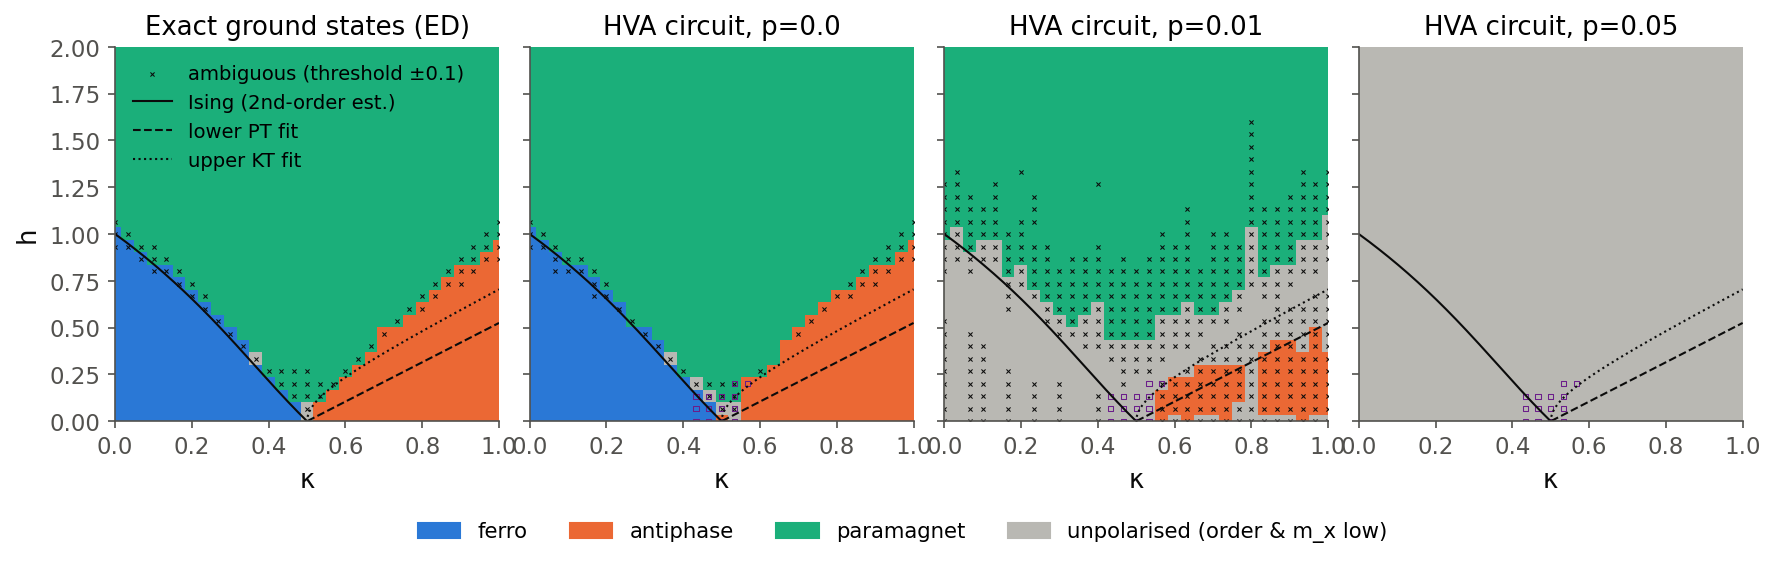
\includegraphics[width=0.86\textwidth]{../results/figures/fig_phase_diagrams_all.png}
\caption{Phase diagrams on the $31\times31$ grid ($N=8$, periodic). From left to right: exact ground states, then the HVA circuit at $p=0$, $0.01$ and $0.05$ with fixed parameters and fixed thresholds. Purple squares mark points where the clean preparation fidelity is below 0.9, and crosses mark threshold-ambiguous points. The curves are the Ising estimate (solid), the lower PT fit (dashed) and the upper KT fit (dotted).}
\label{fig:phases}
\end{figure*}
\begin{figure*}[b]
\centering
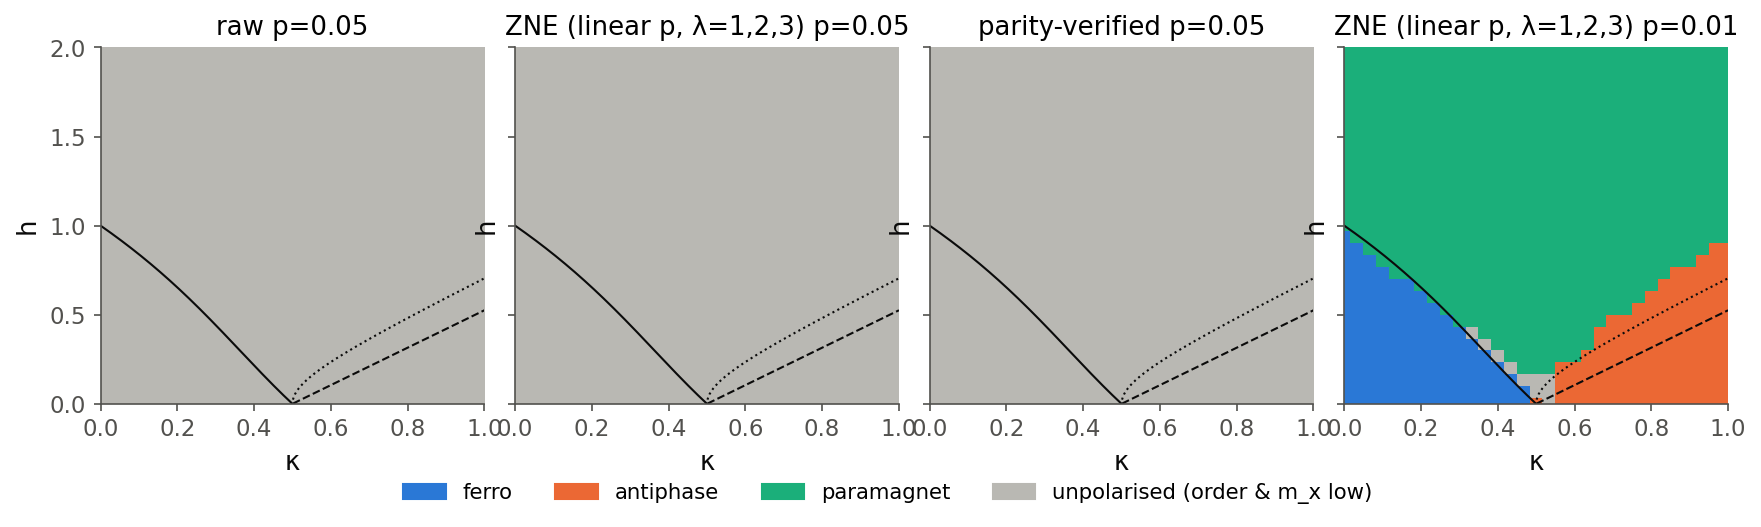
\includegraphics[width=0.5\textwidth]{../results/figures/fig_mitigation_diagrams.png}
\caption{Error mitigation with fixed thresholds. From left to right: the raw map at $p=0.05$, zero-noise extrapolation at $p=0.05$, parity verification at $p=0.05$, and zero-noise extrapolation at $p=0.01$ (Richardson, $\lambda=1,2,3$). Extrapolation restores the $p=0.01$ diagram almost fully, while at $p=0.05$ no usable signal remains.}
\label{fig:mit}
\end{figure*}

\subsection{Finite-size behaviour}
The boundary between the ferromagnet and the paramagnet is almost independent of system size and follows the Ising estimate. At $\kappa=0.2$ the fidelity-susceptibility peak moves from 0.616 at $N=8$ to 0.629 at $N=12$, towards the DMRG value of 0.639 reported in [S10]; the second-order estimate is 0.653. The antiphase boundary, by contrast, drifts strongly with size. At $\kappa=0.75$ the order crossing falls from 0.562 at $N=8$ to 0.432 at $N=12$, approaching the KT fit at 0.423 from above. The ring with $N=10$ cannot hold a period-4 pattern and is visibly anomalous: at $\kappa=0.6$ its crossing sits at 0.397, against 0.244 for $N=8$ and 0.164 for $N=12$. This is a commensurability effect of the finite ring, not physics of the thermodynamic limit.

\subsection{Floating phase}
At $N=12$ the half-chain entropy of the pure ground state peaks close to the KT fit at $\kappa=0.75$ and $\kappa=0.9$, and the antiphase boundary drifts towards the KT line as $N$ grows. Both observations are compatible with a critical region. However, the dominant wavevector $q^*$ stays locked at $\pi/2$ between the PT and KT fits at every size we can reach. The only jumps in $q^*$ occur above the KT line, inside the modulated paramagnet [S10], and the momentum resolution of $\Delta q=\pi/6$ at $N=12$ cannot resolve an incommensurate modulation. We therefore do not claim a floating phase [S12, S23]. As a consistency check rather than an independent validation, a label-free $k$-means clustering on $(S(q)/N,\,m_x)$ reproduces the clean rule labels at 99.1\% of points.

\section{Noise: effects, magnitude and mechanism}

\begin{table*}[t]
\centering
\caption{Boundary positions and noise-induced shifts for the HVA circuit. $h_T$ is the fixed-threshold crossing and $h_D$ the position of the maximum of $-dO/dh$. The grid step is 0.067; the seed-to-seed spread of $\delta h_D$ at $p=0.01$ has median 0.011 and maximum 0.038. The full table for all 31 values of $\kappa$ is in the repository.}
\label{tab:shifts}
\small
\begin{tabular}{@{}l l r r r r r c@{}}
\toprule
$\kappa$ & Order & $h_T^{\rm ED}$ & Prep.\ bias & $h_D(0)$ & $\delta h_D\,(p{=}0.01)$ & $\delta h_D\,(p{=}0.05)$ & $h_T$ at $p{=}0.01$ \\
\midrule
0.2 & ferro & 0.685 & $-0.000$ & 0.653 & $+0.027$ & $+0.64^{\dagger}$ & absent \\
0.3 & ferro & 0.487 & $-0.016$ & 0.469 & $+0.015$ & $+0.19$ & absent \\
0.4 & ferro & 0.246 & $+0.000$ & 0.248 & $+0.003$ & $+0.006$ & absent \\
0.7 & anti  & 0.467 & $+0.018$ & 0.477 & $-0.001$ & $-0.004$ & absent \\
0.8 & anti  & 0.650 & $+0.024$ & 0.672 & $+0.003$ & $+0.045$ & absent \\
0.9 & anti  & 0.809 & $+0.004$ & 0.723 & $+0.000$ & $+0.098$ & absent \\
\bottomrule
\multicolumn{8}{@{}l}{\footnotesize $^{\dagger}$ Unreliable: the order signal at $p=0.05$ is too small to locate a derivative peak.}
\end{tabular}
\end{table*}

\subsection{Noise level $p=0.01$}
The order parameters contract to a median of 0.60 of their clean values, compared with 0.65 if every target hit acted as end-of-circuit noise. The contraction depends on the phase. In the limit $h\to0$, $O_F$ at $\kappa=0.2$ drops from 1.00 to 0.37, whereas $O_A$ at $\kappa=0.9$ drops only to 0.59. Under the fixed threshold the ferromagnet disappears entirely: none of the points that exact diagonalisation labels ferro keep their label, while 46\% of antiphase points and 89\% of paramagnet points survive. Wherever a threshold crossing does survive it moves to lower $h$, by 0.04 to 0.48. This has the same sign as the exact first-order prediction $-p\,\partial_pO/\partial_hO$ but is 1.5 to 4 times larger, because the response is already nonlinear at this noise level. The boundaries defined by derivative peaks, on the other hand, barely move (Table~\ref{tab:shifts}): the median $|\delta h|$ is 0.005, and 28 of the 31 rows stay within 0.03, which is half a grid step. The exceptions are $\kappa=0.13$ and $0.27$, which shift by $+0.04$, and $\kappa=0.93$, which shifts by $-0.12$. This is the behaviour that [S28] predicts for a near-uniform rescaling of the observables, and accordingly the relative-dominance map at $p=0.01$ agrees with the clean exact-diagonalisation map at 97\% of points, compared with 99\% at $p=0$.

\subsection{Noise level $p=0.05$}
At this noise level the state is essentially maximally mixed: the median purity is 0.0047, against 0.0039 for $I/2^8$. Every point is unpolarised under the fixed thresholds. In the relative-dominance map it is the paramagnet that shrinks, because $m_x$ keeps only 16\% of its clean value and hence $m_x^2$ keeps about 2.6\%, while the order parameters keep a median of 8.5\%.

\subsection{Mechanism from exact channel-insertion sums}
We evaluated the first-order response $\partial_p\langle O\rangle=\sum_g{\rm Tr}\{O_g\,\mathcal L_t(\rho_g)\}$ one channel location at a time [S28]. For the ferromagnetic state $d\ln O_F/dp=-99$, for the antiphase $d\ln O_A/dp=-69$, and for $m_x$ in the paramagnet the value lies between $-32$ and $-48$. The value that end-of-circuit noise would give for pair correlators is $-43$. Errors that occur mid-circuit are carried through the later CNOT--RZ--CNOT gadgets and damage the $ZZ$ order more than errors at the end of the circuit would. The early layers contribute the most: for the ferro point, $dO_F/dp$ receives $-27$ from layer 1 and $-17$ from layer 4. One consistent reading of why the ferromagnet is the most fragile phase is that its GHZ-like finite-ring ground state loses all $N(N-1)$ positive correlators in $O_F$ to a single propagated $X$ or $Y$ error, whereas $O_A$ mixes signs and the damage partly cancels. This ranking is specific to this circuit and to these diagnostics, and it reverses the organiser's hypothesis [S01]. The noise does not change the spectrum of the Hamiltonian; what these maps show is the degradation of the prepared state.

\subsection{Depth trade-off}
We repeated the fixed-parameter experiment with $L=1$ to $4$ layers on four cuts in $\kappa$. The clean error $\langle|O-O^{\rm ED}|\rangle_h$ falls with depth while the noise error grows with it, so the best depth shrinks as $p$ grows. The antiphase is already accurate at $L=2$, with a clean error of 0.024 at $\kappa=0.8$, and $L=2$ remains the best depth there at both $p=0.01$ and $p=0.05$. The ferromagnet needs $L=4$ to be accurate, since its error at $L=2$ is 0.17, and at $p=0.01$ its best depth is $L=3$. The ferromagnetic state therefore needs the full depth and carries the most noise channels, which is a second reason it suffers most.

\section{Error mitigation}

\subsection{Zero-noise extrapolation}
We ran Richardson extrapolation on every correlator $C_{ij}$ and every $\langle X_i\rangle$ evaluated at $\lambda p$ for $\lambda=1,2,3$ (linear noise scaling), holding out the $p=0$ truth, and rebuilt $S(q)$ before classifying. At $p=0.01$ this is effective (Figure~\ref{fig:mit}): the median $|\Delta C_{ij}|$ falls from 0.063 to 0.011, $|\Delta m_x|$ falls from 0.26 to 0.023, and label agreement with the clean circuit rises from 70\% to 98\%. The threshold boundaries return to within $|\delta h|\le0.09$ with a median of 0.03; at $\kappa=0.93$, for example, the shift goes from $-0.48$ to $-0.04$. The price is a variance-amplification factor of $\sum\gamma^2=19$. At $p=0.05$ zero-noise extrapolation fails for both linear and composed-channel scaling, because the remaining signal is about 1\% and the extrapolation has to reach out to $p=0.15$.

\subsection{Parity verification}
Post-selecting on the parity operator $P=\prod_i X_i$ accepts 71\% of the weight at $p=0.01$ and 51\% at $p=0.05$. It lowers the error in $C_{ij}$ only from 0.063 to 0.053, because most errors stay inside the even-parity sector.

\subsection{Noise-aware re-optimisation}
As a separate protocol on the cuts $\kappa=0.2$, $0.3$, $0.7$ and $0.8$, with 8 values of $h$ each, we minimised ${\rm Tr}(H\rho_p)$ with exact gradients through the channels. This lowers the noisy energy by 0.2 to 1.0 per cut, but the order parameters move by only $-0.016$ to $+0.028$ and their error against exact diagonalisation is unchanged; at $\kappa=0.8$ and $p=0.01$, for example, it goes from 0.225 to 0.198. The optimiser gains energy mainly through $m_x$, which rises by $+0.03$ to $+0.09$, by leaving the ground state: at $\kappa=0.2$, $h=0$ the clean energy of the re-optimised parameters is $-5.83$, against $-6.40$ for the true ground state. Energy-optimal noisy states are therefore not diagnostic-optimal.

\section{Conclusions and limitations}
The clean phase diagram is reproduced accurately on rings of 8 to 12 sites. For a symmetric circuit accurate enough to represent these ground states, which costs 128 CNOTs, noise at $p=0.01$ already removes the ferromagnet under fixed thresholds while the boundary positions defined by derivatives stay put, and $p=0.05$ leaves no usable signal at all. Zero-noise extrapolation recovers the $p=0.01$ map almost fully. The limitations are the small system sizes, the approximate overlay curves, the masking of the $\kappa\approx0.5$ region for preparation quality, the use of the fixed-parameter protocol on the full grid with re-optimisation only on cuts, and the absence of shot noise in these exact simulations.

\vspace{0.6ex}
{\scriptsize\noindent\textbf{References.} Full entries are in the repository's literature notes.
[S01] Organiser handout; [S07] starter-kit audit; [S10] Beccaria, Campostrini, Feo, PRB 73, 052402 (2006); [S12] Cea et al., arXiv:2402.11022 (2024); [S13] Beccaria, Campostrini, Feo, PRB 76, 094410 (2007); [S19] Temme, Bravyi, Gambetta, PRL 119, 180509 (2017); [S21] Bonet-Monroig et al., PRA 98, 062339 (2018); [S23] Sandvik, AIP Conf.\ Proc.\ 1297, 135 (2010); [S28] our channel-response derivation; [S30] Wecker, Hastings, Troyer, arXiv:1507.08969 (2015). Tools: PennyLane 0.44.1, NumPy, SciPy, Matplotlib.\par}

\end{document}
